\documentclass[letterpaper]{article}
\usepackage{times}
\usepackage{helvet}
\usepackage{courier}

%═══════════════════════════════════════════
% Math packages
%═══════════════════════════════════════════
\usepackage{amssymb,amsthm,amsmath}
\usepackage{mathtools}
\usepackage{proof}
\usepackage{bussproofs}
\usepackage{marvosym}
\usepackage{thmtools}
\usepackage{thm-restate}
\DeclarePairedDelimiter{\ceil}{\lceil}{\rceil}


%═══════════════════════════════════════════
% Formatting, margins, and spacing packages
%═══════════════════════════════════════════
\usepackage{microtype}
\usepackage{enumitem}
\frenchspacing
\setlength{\pdfpagewidth}{8.5in}
\setlength{\pdfpageheight}{11in}
\setlist[enumerate]{itemsep=0mm}
\setlist[itemize]{itemsep=0mm}
\setlist[description]{itemsep=0mm}

%═══════════════════════════════════════════
% Graphics packages
%═══════════════════════════════════════════
\usepackage{tikz}
\usetikzlibrary{positioning,calc,arrows.meta,shapes.geometric,fit, backgrounds}

%═══════════════════════════════════════════
% Environments
%═══════════════════════════════════════════
\theoremstyle{definition}
\newtheorem{definition}{Definition}
\newtheorem{theorem}{Theorem}
\newtheorem{lemma}[theorem]{Lemma}
\newtheorem{claim}{Claim}
\newtheorem{postulate}{Postulate}
\newtheorem{corollary}{Corollary}
\newtheorem{proposition}{Proposition}
\newtheorem{example}{Example}
\newtheorem{remark}[theorem]{Remark}
\newtheorem*{aside}{Quick Aside}
\newtheorem*{question}{Question}
\newenvironment{sketch}{\begin{proof}[Proof Sketch]}{\end{proof}}

%═══════════════════════════════════════════
% References, Links, and Color
%═══════════════════════════════════════════
% AAAI requires that color is never used in text
% (can be used in diagrams carefully though!)
\usepackage{biblatex}
\addbibresource{references.bib}
\usepackage{xcolor}
\definecolor{mygreen}{RGB}{107,203,119}
\definecolor{myblue}{RGB}{77, 150, 255}
\usepackage[colorlinks,allcolors=myblue]{hyperref}

%═══════════════════════════════════════════
% Custom Commands, General Use
%═══════════════════════════════════════════
\newcommand{\key}[1]{\emph{#1}}
\newcommand{\Rat}{\mathbb{Q}}
\newcommand{\Nat}{\mathbb{N}}
\newcommand{\State}{\mathsf{State}} 
\newcommand{\semantics}[1]{[\![\mbox{\em $ #1 $\/}]\!]}
\newcommand{\Model}{\mathcal{M}}
\newcommand{\Nodel}{\mathcal{N}}
\newcommand{\lang}{\mathcal{L}}
\newcommand{\uplang}{\mathcal{L}^\ast}
\newcommand{\vocab}{\mathcal{V}}
\newcommand{\wocab}{\mathcal{W}}
\newcommand{\set}[1]{\{ #1 \}}
\newcommand{\proves}{\vdash}
\renewcommand{\o}{\cdot}
\newcommand{\orr}{\vee}
\newcommand{\andd}{\wedge}
\newcommand{\nott}{\neg}
\newcommand{\bigandd}{\bigwedge}
\newcommand{\quadiff}{\quad \mbox{ iff } \quad}
\newcommand{\rem}[1]{\relax}
 \newcommand{\NP}{\mbox{\sc np}}
\newcommand{\axiom}{\textsc}
\newcommand*{\bigchi}{\mbox{\Large$\chi$}}% big chi
\newcommand{\degree}[1]{\mathrm{deg}(#1)}
\newcommand{\preds}[1]{\mbox{preds}(#1)}
\newcommand{\layer}[1]{\mathsf{layer}(#1)}
\newcommand{\activ}[2]{\mathsf{activ}_{#1}(#2)}
\newcommand{\layerNoArgs}{\mathsf{layer}}

\newcommand{\negweightscore}[1]{\mathsf{nws}(#1)}
\newcommand{\minscore}{\mathsf{mnws}}
\newcommand{\numiterations}{\mathsf{iter}}

%═══════════════════════════════════════════
% Custom Commands, Hebbian Learning
%═══════════════════════════════════════════
\newcommand{\AllNets}{\mathsf{Net}}
\newcommand{\Net}{\mathcal{N}}
\newcommand{\op}{\mathsf{op}}
\newcommand{\Prop}{\mathsf{Prop}}
\newcommand{\Reach}{\mathsf{Reach}}
\newcommand{\Hebb}[2]{\mathsf{Hebb}(#1, #2)}
\newcommand{\HebbNoArgs}{\mathsf{Hebb}}
\newcommand{\Hebbstar}[2]{\mathsf{Hebb}^*(#1, #2)}
\newcommand{\HebbstarNoArgs}{\mathsf{Hebb}^*}
\newcommand{\hebbweight}{W_\mathsf{Hebb}}
\newcommand{\hebbstarweight}{W_{\mathsf{Hebb}^*}}

\newcommand{\Typ}[1]{\textrm{\textup{\textbf{T}}} #1}
\newcommand{\Know}[1]{\textrm{\textup{\textbf{K}}} #1}
% \newcommand{\Know}[2]{\textrm{\textup{\textbf{K}}}(#1, #2)}
\newcommand{\KnowNoArgs}{\textrm{\textup{\textbf{K}}}}
\newcommand{\TypNoArgs}{\textrm{\textup{\textbf{T}}}}
% \newcommand{\Hebbop}[1]{[#1]_\textrm{\textup{hebb}\:}}
% \newcommand{\Hebbop}[1]{[#1]_{\HebbstarNoArgs}\:}
\newcommand{\Hebbop}[1]{[#1]}
\newcommand{\Update}[1]{[#1]}
\newcommand{\Best}[1]{[\mathsf{best}] #1}
\newcommand{\BestNoArgs}{[\mathsf{best}]}
\newcommand{\Believe}[2]{\textrm{\textup{\textbf{K}}}^{#1} #2}

\newcommand{\diaTyp}[1]{\langle \textrm{\textup{\textbf{T}}} \rangle #1}
\newcommand{\diaKnow}[1]{\langle \textrm{\textup{\textbf{K}}} \rangle #1}
% \newcommand{\diaKnow}[2]{\langle \textrm{\textup{\textbf{K}}} \rangle(#1, #2)}
\newcommand{\diaTypNoArgs}{\langle \textrm{\textup{\textbf{T}}} \rangle}
\newcommand{\diaKnowNoArgs}{\langle \textrm{\textup{\textbf{K}}} \rangle}
% \newcommand{\diaHebbop}[1]{\langle #1\rangle_\textrm{\textup{hebb}}}
\newcommand{\diaHebbop}[1]{\langle #1\rangle}
\newcommand{\diaUpdate}[1]{\langle #1\rangle}
\newcommand{\diaBest}[1]{\langle \mathsf{best}\rangle #1}

%═══════════════════════════════════════════
% Beginning of Notes
%═══════════════════════════════════════════
\begin{document}

\section*{Problem Statement}

Consider the dynamic epistemic language
\[
    p \mid \neg \varphi \mid \varphi \land \psi \mid \Know{\varphi} \mid \Typ{\varphi} \mid \Update{P} \varphi
\]
$\KnowNoArgs$ is knowledge.  $\TypNoArgs$ is more interesting --- $\Typ{\varphi}$ says that the current world is `minimal' or `most typical' over worlds satisfying $\varphi$.  (As far as I can tell, this is not quite the same as the $\BestNoArgs$ operator, see Remark 10 in \cite{van2007beliefrevision}).  $\Update{P}$ is some dynamic update given by $\Model \to \Model^\star_P$ (this is a free variable; the problem will be to find the right update).

For the static part of the logic, choose your favorite semantics --- plausibility models, evidence models, etc.  For now, I'll take Johan's approach from \cite{van2011logical}, which I've been using as a desk reference for all this.  Let's assume we have a single-agent plausibility model, with an extra accessibility relation $R$ for knowledge: $\Model = \langle W, R, \leq, V \rangle$.  $\leq$ is uniform over all states; we do not have a different plausibility relation $\leq_s$ for each state.  As usual, $x \leq y$ reads ``the agent finds x at least as plausible as y.''

\begin{definition}
    The semantics are given by
    \[
    \begin{array}{lcl}
        \Model, w \Vdash p & \mbox{ iff } & w \in V(p)\\
        \Model, w \Vdash \neg \varphi & \mbox{ iff } & \Model, w \not \Vdash \varphi\\
        \Model, w \Vdash \varphi \land \psi & \mbox{ iff } & \Model, w \Vdash \varphi \mbox{ and } \Model, w \Vdash \psi\\
        \Model, w \Vdash \Know \varphi & \mbox{ iff } & \mbox{for all } u \mbox{ with } w{R}u, \Model, u \Vdash \varphi \\
        \Model, w \Vdash \Typ{\varphi} & \mbox{ iff } & w \mbox{ is } {\leq}\mbox{-minimal over } \set{u \mid \Model, u \Vdash \varphi} \\
        \Model, w \Vdash \Update{P} \varphi & \mbox{ iff } & \Model^\star_P, w \models \varphi
    \end{array}
    \]
\end{definition}

I will use the shorthand $\semantics{\varphi}_\Model =   \set{u \mid \Model, u \Vdash \varphi}$, and drop $\Model$ when it's understood from context.

Iterated Hebbian learning, formalized as a dynamic update on neural network models, can be reduced to this language \cite{kisby2024hebbian}.  The reduction axioms are:
\[
    \begin{array}{lcll}
        \Hebbop{P} p & \leftrightarrow & p \quad \quad \mbox{ for propositions } p \\
        \Hebbop{P} \neg \varphi & \leftrightarrow & \neg \Hebbop{P} \varphi\\
        \Hebbop{P} (\varphi \land \psi) & \leftrightarrow & \Hebbop{P} \varphi \land \Hebbop{P} \psi \\
        \Hebbop{P} \Know{\varphi} & \leftrightarrow & \Know{\Hebbop{P} \varphi}\\
        
        \Hebbop{P} \Typ{\varphi} & \leftrightarrow & 
        \Typ{(\Hebbop{P}\varphi \land (\Typ{P \lor \Know{(\Typ{P} \lor \Typ{\Hebbop{P}\varphi})}}))}
    \end{array}
\]
I would like to understand what neural network updates are doing ``classically,'' i.e.\ for each neural network update, what is an ``equivalent'' update over possible worlds / plausibility / evidence models?  In this case, my question for you is:
\begin{question}
    Is there a dynamic model update (over your classical model of choice) that satisfies these reduction axioms?
\end{question}
I've been stuck on this since November (I probably should have reached out sooner).

\section*{Progress So Far}

I've somewhat misled you by talking in terms of plausibility models.  In fact, the reduction above is \emph{invalid} for relational plausibility upgrades.

\begin{proposition}
    No plausibility upgrade $\Model \to \Model^\star$,  where $\Model = \langle W, \leq, V \rangle$ and $\Model^\star = \langle W, \leq^\star, V \rangle$ can make the axioms for iterated Hebbian learning valid.
\end{proposition}
\begin{proof}
    Let $\Model \to \Model^\star$ be any plausibility upgrade.  I will show that the very last axiom cannot hold for all $\Model, w$; specifically, this propositional instance will fail:
    \[
        \Update{p} \Typ{q} \leftrightarrow 
        \Typ{(q \land (\Typ{p} \lor \Know{(\Typ{p} \lor \Typ{q})}))}
    \]
    Let's construct a $\Model$ and $w$ that make it fail.  Let $\Model$ be

    \begin{center}
    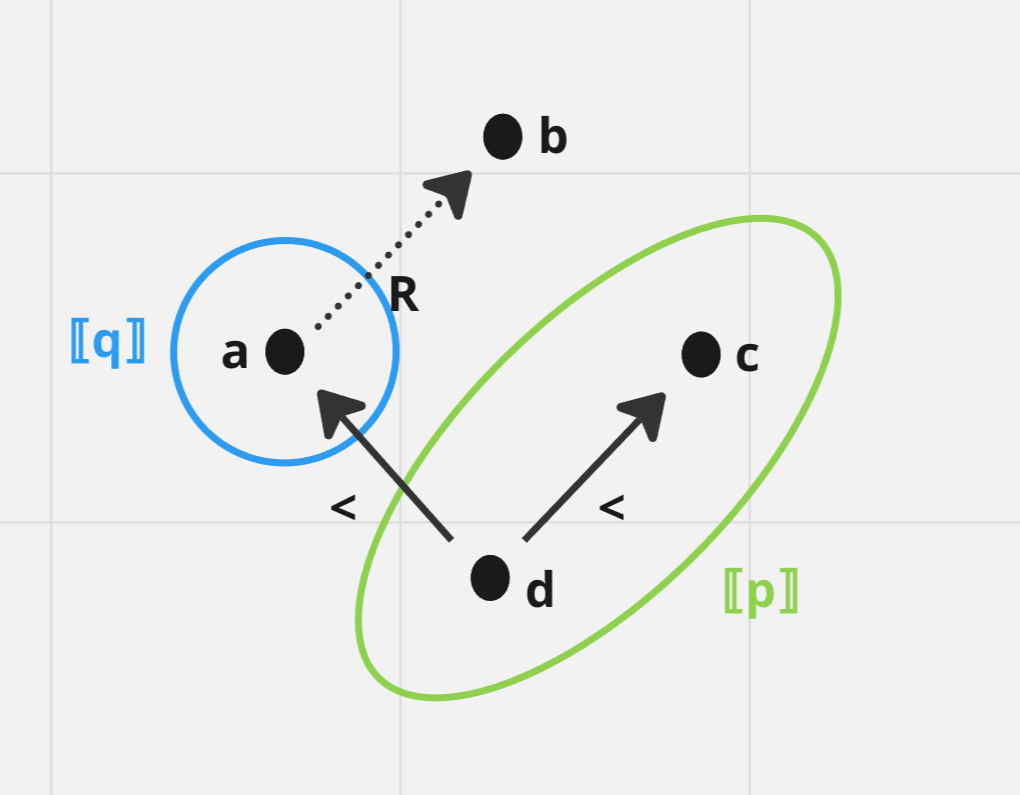
\includegraphics[scale=0.18]{4-22-24-mockup.png}
    \end{center}

    Note that $\Model \to \Model^\star$ only modifies $\leq$.  This means that $\semantics{q}_\Model = \semantics{q}_{\Model^\star_p}$.  So in particular, $\semantics{q}_{\Model^\star_p}$ is finite and nonempty.  So there is some $w$ that is ${\leq}$-minimal over $\semantics{q}_{\Model^\star_p}$.  So $\Model, w \Vdash \Update{p} \Typ{q}$.

    WHOOPS, THINK ABOUT IT MORE 
    
    I will now show that no choice of $w$ can satisfy $\Typ{(q \land (\Typ{p} \lor \Know{(\Typ{p} \lor \Typ{q})}))}$.  Well, the only $u$ such that $\Model, u \Vdash q$ is $a$.  But $\Model, a \not \Vdash \Typ{p}$ (since $a$ is not a $\leq$-minimal element of $\semantics{p}$).  Additionally, there \emph{is} $b$ with $a{R}b$ such that $b$ is not a $\leq$-minimal element of either $\semantics{p}$ \emph{or} $\semantics{q}$.  So $\Model, b \not \Vdash \Typ{p} \lor \Typ{q}$, and thus $\Model, a \not \Vdash \Know{\Typ{p} \lor \Typ{q}}$.
    
    
    --------------------------

    I will now show that $\Model, w$ does not satisfy either of the disjuncts.  In particular:
    \begin{enumerate}
        \item $\Model, w \not \Vdash \Typ{(p \land q)}$, since $\semantics{p} \cap \semantics{q} = \emptyset$ (and so there is no ${\leq}$-minimal element of $\semantics{p} \cap \semantics{q}$).  So $\Model, w$ does not satisfy the left disjunct.
        
        \item $\Model, w \not \Vdash \neg\Diamond(p \land \diaTyp{q})$, since there \emph{does} exist $b$ such that $\Model, b \Vdash p \land \diaTyp{q}$ (observe: $b \in \semantics{p}$ and $b$ is not minimal in $\semantics{q}^\complement$).  So $\Model, w$ does not satisfy the right disjunct.\qedhere
    \end{enumerate}
\end{proof}

The crucial step of this proof is finding this ${\leq}$-minimal $w$ in $\semantics{q}_{\Model^\star_p}$.  Note that this step does not rely on the well-foundedness of $\leq$ --- we can construct a similar model that is not well-founded if we like.  But it \emph{does} rely on the fact that $\Update{p} q \leftrightarrow q$ is valid: re-ordering $\leq$ \emph{cannot add or remove} elements from $\semantics{q}$.  In particular, the proof would break if our update could make $\semantics{q}$ empty or make $\semantics{q}$ include an infinite descending chain.  (But I can't figure out an update that would do these in the right way\ldots)

\begin{corollary}
    No plausibility upgrade can make Axiom B valid.
\end{corollary}

The proof is a simple extension of the above proof, replacing $p$ with $\diaTyp{p}$.  We can show the same for axiom C, by modifying the construction slightly.

\begin{proposition}
    No plausibility upgrade can make Axiom C valid.
\end{proposition}
\begin{proof}
    Consider the propositional instance of Axiom C:
    \[
        \Update{p} \Typ{q} \leftrightarrow 
        \Typ{(q \land (\Typ{p} \lor \Know{(\Typ{p} \lor \Typ{q})}))}
    \]
    Let $\Model \to \Model^\star$ be any plausibility upgrade.  This time, let $\Model$ be
    
    [PICTURE]

    Again, $\Model \to \Model^\star$ only modifies $\leq$, and in particular $\semantics{q}_{\Model^\star_p}$ is finite and nonempty.  So there is some $w$ that is ${\leq}$-minimal over $\semantics{q}_{\Model^\star_p}$.  So $\Model, w \Vdash \Update{p} \Typ{q}$.  
    
    TODO
\end{proof}

\printbibliography

\end{document}

% I'll also assume for now that $\leq$ is well-founded (there are no infinite descending chains).
% I would like your help with a problem I'm stuck on, if you don't mind giving it some thought.  I ran into this issue in my work on neural network update, but the question I have for you are about epistemic/plausibility models, not neural network models.  I'll try to state the question as cleanly as I can, and then if you're interested in knowing \emph{why} I care about all this I'll be happy to explain face-to-face.
